\documentclass{beamer}
\usepackage{multicol}
\usepackage{natbib} 
\def\newblock{\hskip .11em plus .33em minus .07em}
\newcommand\independent{\protect\mathpalette{\protect\independenT}{\perp}} 
\def\independenT#1#2{\mathrel{\rlap{$#1#2$}\mkern2mu{#1#2}}} 
%\usepackage{beamerthemeBerkeley}
% Use either the one above or the one below
\usetheme{Hannover}

\title{The Bootstrap}
%\author{	Mike Higgins from F. Daniel Hidalgo's notes\\ }
%\date{\today}

\begin{document}

\frame{\titlepage}

%\section[Outline]{}
%\frame{\tableofcontents}

%Sample median
%bias
%hypothesis test
%confidence intervals

%regression
%parametric, non-parametric

%loess
%time series

\frame{
	\frametitle{Motivation}
        \begin{itemize}
          \item<1-> Suppose we take a sample of 1,000 people from a large population.
            We are interested in estimating, say, the average height of the people in the population.
          \item<1->
            Suppose population heights have mean $\mu$ and standard deviation $\sigma$.
            We are interested in estimating $\mu$.
          \item<1-> We know (by the CLT) that the sample average should be 
            approximately normal with mean $\mu$ and variance $\sigma^2/1000$. \\
            We can use this fact to obtain standard errors and form confidence intervals or
            perform hypothesis tests.\\  
            This is an easy inference problem.
          \item<2-> What if we weren't interested in the population mean, but the population
            median?
          \item<2-> Depending on the population, there may not be a ``nice formula''
            for the distribution sample median.  \\
            This is a harder inference problem.
          \end{itemize} 
}
\frame{
	\frametitle{Ideal Scenario}
        \begin{itemize}
          \item<1-> To estimate the distribution of the sample median,
            we could take samples of 1,000 people over and over and over and over again.
          \item<1->  For each sample of 1,000 people, find the sample median.
          \item<1-> Draw a histogram of these sample medians: 
            should be close to the true distribution.          
          \end{itemize} 
}
\frame{
	\frametitle{Gamma distribution:}
	\begin{center}
        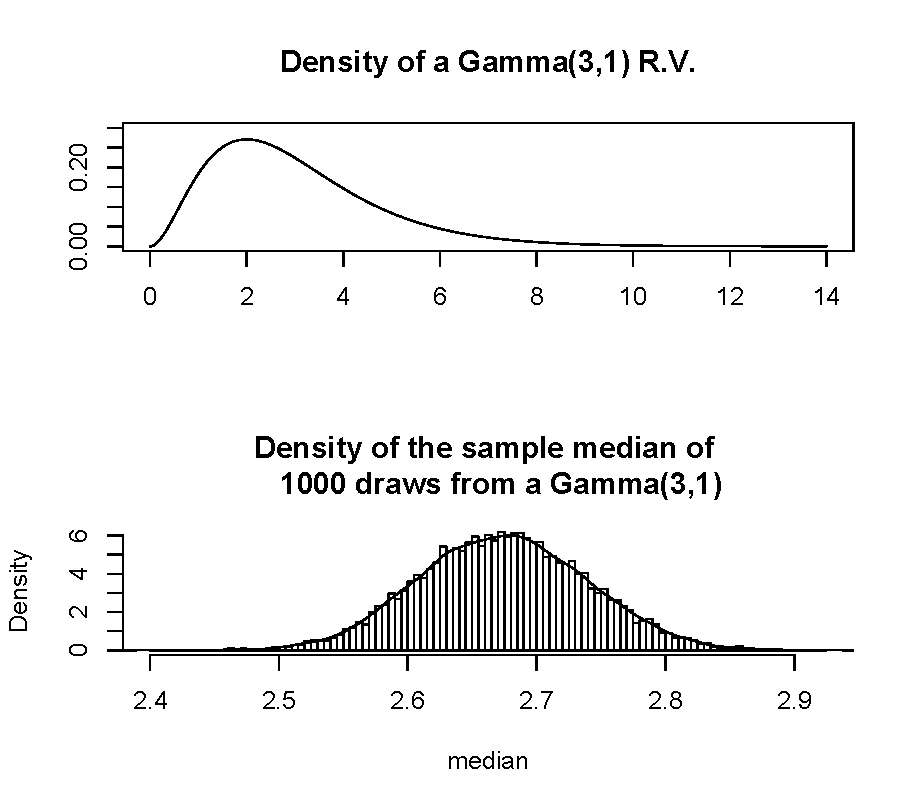
\includegraphics[width = .9\textwidth]{densityandmedian.pdf}
        \end{center}
}
\frame{
	\frametitle{Bootstrap Idea:}
        \begin{itemize}
          \item<1-> In practice, we only have one sample.  
            Impossible to sample many times to obtain a sampling distribution.
          \item<2->  HOWEVER, if we sampled well, 
            the data from our sample should
            be close in distribution to the data from the population.
            (Key idea: Empirical distribution obtained by the sample
              converges to the true distribution)
          \item<2->  Resampling (with replacement) from our sample many, many times
            is ALMOST like resampling from the entire population. \\
          \item<3->  For many statistics, we can get close to the 
            sampling distribution this way.
          \end{itemize} 
}
\frame{
   \frametitle{Bootstrap for Gamma:}
   \begin{center}
        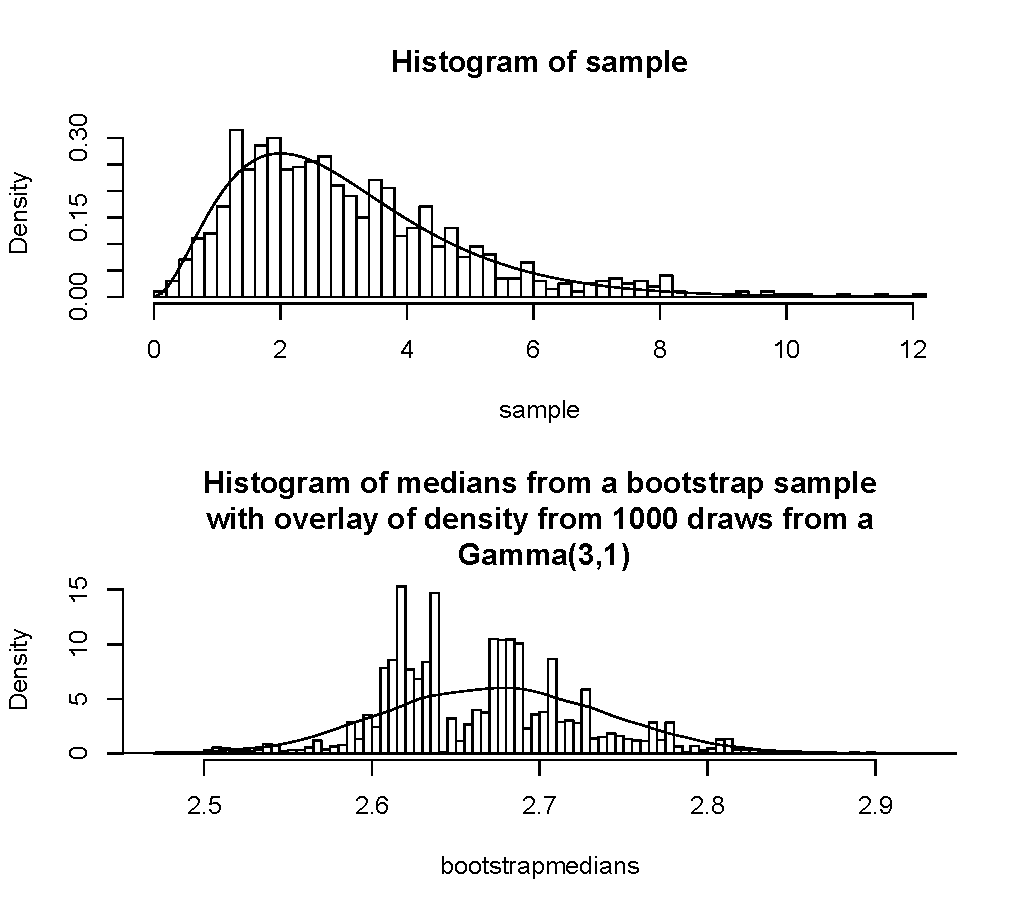
\includegraphics[width = .9\textwidth]{densityandmedianboot.pdf}
        \end{center}
}
\frame{
	\frametitle{Estimation of standard errors:}
        \begin{itemize}
        \item<1-> Let $\mathbf{x}$ denote the original sample of $n$ units.
          Let $\hat\beta$ denote the median (or any other parameter of interest)
          of the sample
        \item<1-> Select (Large) $B$ independent bootstrap samples
          $\mathbf{x^{*1},x^{*2},...,x^{*B}}$, each consisting of $n$
          data values draw \textbf{with replacement} from $\mathbf x$.
        \item Compute the median for each sample.
          Let $\hat\theta^*_1,\ldots,\hat\theta^*_B$ denote these medians.
          Let $\bar \theta^* = \frac{1}{B}\sum  \hat\theta^*_i$ denote the
          average of these medians.
        \item Estimate the standard error for the sample median 
          by taking the 
          standard deviation of the $B$ bootstrap medians.
	$$
	\widehat{\textrm{se}}_B =\left \{ \sum_{i=1}^B[\hat \theta^*_i - \bar
	\theta^*]^2/(B-1)\right \}^{1/2}.
	$$
	\end{itemize}
}
\frame{
	\frametitle{The Bootstrap Algorithm for SE}
     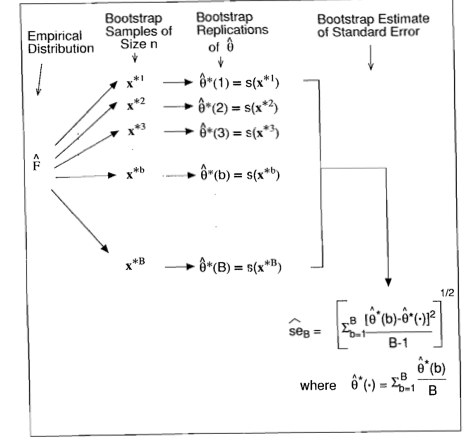
\includegraphics[width=8cm]{bootstrap_algorithm_se.png}  
}
\frame{
	\frametitle{Bootstrap confidence intervals:}
	\begin{itemize}
        \item<1-> Bootstrap confidence intervals are easy too!
        \item<1-> Suppose we want to find a $1-\alpha$ confidence interval.
        \item<1-> We can form a bootstrap confidence interval by finding the
          $\alpha/2$ and the $(1-\alpha/2)$ percentile of the bootstrap medians
          $(\hat\theta^*_1,\ldots,\hat\theta^*_B)$.
        \item<2-> For example, if we took 10,000 bootstrap samples, the
          if we denote $\hat\theta^*_{(i)}$ as the $i^{\text{th}}$ largest bootstrap
          median, a 95\% bootstrap confidence interval would be
          $[\hat\theta^*_{(251)},\hat\theta^*_{(9750)}]$.
     \end{itemize}
}
\frame{
   \frametitle{Bootstrap CI:}
   \begin{center}
        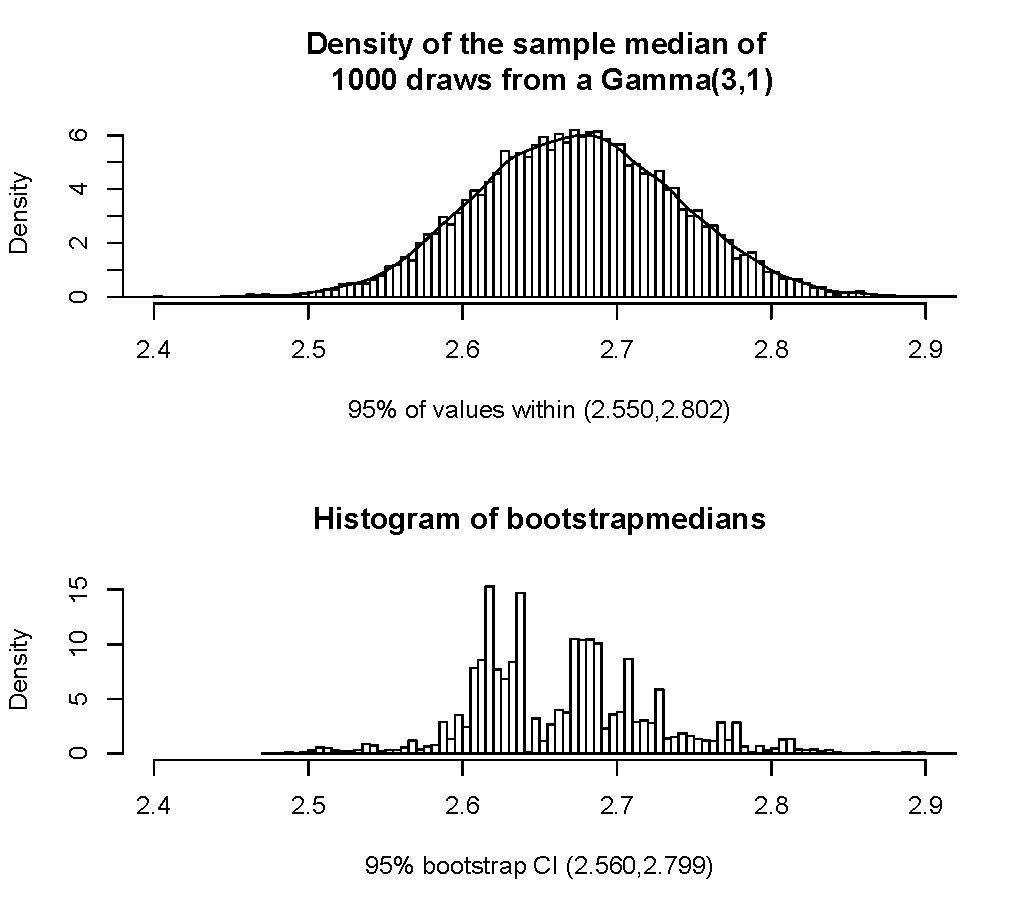
\includegraphics[width = .9\textwidth]{comprealandboot.pdf}
        \end{center}
}
\frame{
	\frametitle{Warnings:}
	\begin{itemize}
        \item<1-> Note: bootstrap estimation is only as good as the data you begin with.
          \begin{itemize}
            \item Median of the distribution: 2.674
            \item Median of sample: 2.668
            \begin{center}
                      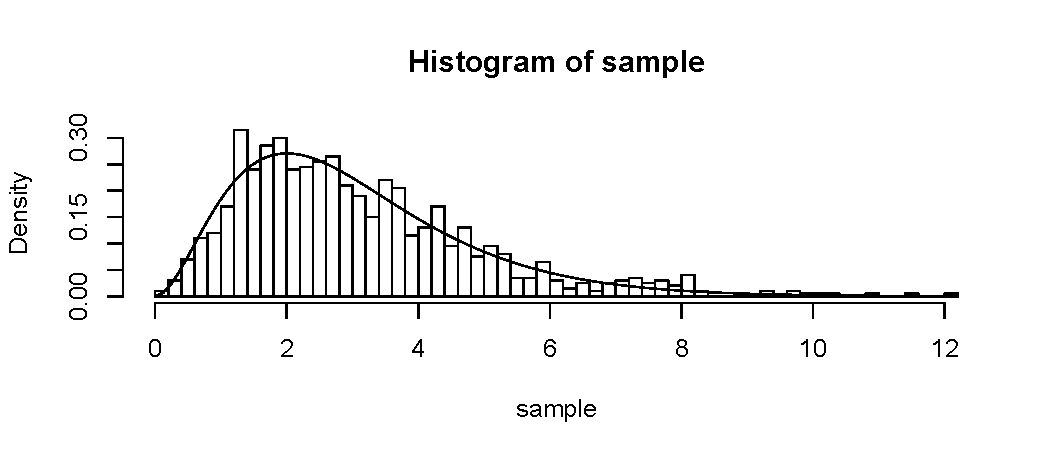
\includegraphics[width = .75\textwidth]{histofsample.pdf}
            \end{center}
           \end{itemize}
        \item<1-> If sample does not look like original distribution, then
          bootstrapping may fail (think Type I Errors).
          There's no good way to check this unless you make an assumption
          about the distribution of the population.
     \end{itemize}
}
\frame{
	\frametitle{Other applications of Bootstrap:}
        \begin{itemize}
        \item<1-> Many possible applications for bootstrap, not just
          finding sampling distributions.
        \item<1-> Find estimates, standard errors, and bias in
          complicated models fitted to data.
          (See \textit{Statistical Models} by David Freedman for some examples)
        \item<1->  Can also be used for testing.
        \item<2->  Key idea: mechanism for resampling has to preserve original 
          structure of data.
        \item<2->  
          For example:  If a set of data points is assumed to be i.i.d., we can
          mimic their distribution by resampling from the data points with replacement.
        \end{itemize}
}
\frame{
	\frametitle{Example: Regression Models}
        \begin{itemize}
        \item<1-> We know the formulas for finding standard errors in
          in regression, but suppose we forgot.
        \item<1->   Suppose we assume the model
          $Y_i=X_i\beta + \epsilon_i$, where the design matrix
          $X$ is fixed and has full rank and the errors 
          $\epsilon_1,\ldots,\epsilon_n$
          are IID with mean 0 and variance $\sigma^2$.
        \item<1-> Now, $Y_i$'s are not i.i.d., but the $\epsilon_i$ are.
          If the $Y_i$ are linear in $X$, the residuals $e_i = Y_i- X_i\hat \beta$ 
          should be close to the actual errors $\epsilon_i$.
         \item<1-> By resampling from the residuals 
          we preserve the randomness structure. 
        \end{itemize}
     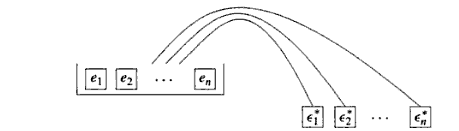
\includegraphics[width=8cm]{bs_reg.png}  
} 

\frame{
	\frametitle{Example: Regression Models}
        \begin{itemize}
          \item<1-> Draw $n $ times at random with replacement from
            this population to get bootstrap errors
            $\epsilon^*_1,\ldots \epsilon^*_n$. These are i.i.d. (because
            you sample them that way).
          \item<1-> Generate the $Y^*_i$:
$$Y^*_i = X_i \hat \beta + \epsilon^*_i$$
	\item<1->  Given $Y^*$ and $X$, can then get the regression estimate
  $\hat \beta^*=(X'X)^{-1}X'Y^*$.
    	\item<2-> Do this over and over to get many, many $\hat\beta^*$.
	\item<2-> Distribution of 
	  $\hat \beta^* - \hat \beta$ is a good 
	  approximation for the distribution of $\hat \beta - \beta$. 
	\item<2->  The empirical covariance 
	  matrix of the $\hat \beta^*$ (computed by actually taking variances
	  and correlations of $\hat\beta^*$ terms) should be close
	  to the thoretical covariance matrix of $\hat \beta$.
        \end{itemize}
}

\frame{
	\frametitle{Example: Kolmogorov-Smirnov}
        \begin{itemize}
          \item<1-> Here is the procedure for computing bootstrap $p$-values
            for the KS test in the Matching package.\\
            (Very similar to permutation tests.)
          \item<1-> Suppose we a treatment group of $m$ units and a control group of $n$.
            Members of each group are selected i.i.d, and units in the treatment group are
            selected independently from the control group.         
          \item<1->  Let $\widehat{KS}$ denote the value of the KS statistic for these groups.
          \item<2-> Under the null hypothesis of a KS test: both groups have the same distribution.
          \item<2-> Let $y_1,\ldots,y_m$ denote the observations from the treated group
            and let $y_{m+1}, \ldots, y_{m+n}$ denote the observations from the control group.
          \item<2-> Under null, the distribution of $(y_1,\ldots,y_m)$ is the same as of
            $(y_{m+1}, \ldots, y_{m+n})$ is the same as $(y_1, \ldots, y_{m+n})$.
        \end{itemize}
}

\frame{
	\frametitle{Example: Kolmogorov-Smirnov}
          To get distribution of KS test statistic under the null hypothesis:
            \begin{enumerate}
             \item Draw $m+n$ observations with replacement from $(y_1, \ldots, y_{m+n})$.
             \item Assign first $m$ observations to ``treatment,'' assign next $n$ to ``control.''
             \item Compute the KS statistic $\widehat{KS}^*$ for this assignment of treatment and control.
             \item Do this many, many, many times to get a distribution of the KS statistic under the null
               hypothesis.
             \end{enumerate}
            The KS bootstrap $p$-value is the proportion of bootstrap trials with a 
             KS statistic $\widehat{KS}^* \geq \widehat{KS}$.
}
\end{document}
